\documentclass{article}
\usepackage{amsmath}
\usepackage[hidelinks]{hyperref}
\usepackage{amssymb}
\usepackage{tikz}

\makeatletter
\renewcommand{\eqref}[1]{%
  \hyperref[#1]{\textup{\tagform@{\ref*{#1}}}}%
}

\begin{document}
\begin{titlepage}
    \vspace{20mm}
    \begin{center}
        \Huge \textbf{Appunti di Intelligenza Artificiale} \\
        \medskip
        \LARGE By \textit{@Thisisfava}\\
        \medskip
        \large 2024/2025
    \end{center}
\end{titlepage}
\newpage
\addcontentsline{toc}{section}{}
\tableofcontents
\newpage
\section{Numeri Complessi}
\paragraph{Definizione.} Il campo complesso $\mathbb{C}$ è la chiusura algebrica di un polinomio di grado $n$ a coefficienti reali.
Un numero $z \in \mathbb{C}$ è definito dall'\textit{unità immaginaria}:
\begin{equation}
    i = j = \sqrt{-1}
\end{equation}

\subsection{Rappresentazioni}
Un complesso $z$, che può essere scritto in diverse forme, viene rappresentato sul \textit{Piano di Gauss}, 
un piano definito dall'asse orizzontale $\mathbb{R}e$ e dall'asse verticale $\mathbb{I}m$
\subsubsection{Coordinate Rettangolari}
Un complesso può essere rappresentato come un punto $\left(x,y\right)$ sul piano di Gauss, con $x$ e $y \in \mathbb{R}$ . La forma che lo rappresenta è la forma \textit{algebrica}:
\begin{equation}
    z = x + jy
\end{equation}
Con $x$ la parte reale (ossia $\mathbb{R}e(z) = x$) e $y$ la parte immaginaria (ossia $\mathbb{I}m(z) = y$)

\subsubsection{Coordinate Polari}
Un complesso $z$ può essere anche rappresentato in \textit{forma polare} sul piano in funzione della lunghezza $\rho$ del vettore che parte dall'origine (ossia il \textit{modulo}) e dell'angolo spazzato $\theta$ (ossia la \textit{fase}).
\begin{equation}
    z = \langle \rho, \theta \rangle = \rho\left(\cos\left(\theta\right) + j\sin\left(\theta\right) \right)
\end{equation}
In realtà, un'altra forma che permette di esprimere un complessi in coordinate polari è la forma \textit{esponenziale}
\begin{equation}
    z = \rho e^{j\theta} = \rho\left(\cos\left(\theta\right) + j\sin\left(\theta\right) \right) 
\end{equation} 


\subsection{Conversioni}
\subsubsection{Polare a Rettangolare}
Dato $z = \langle\rho, \theta\rangle $
\begin{equation}
    \begin{cases}
        x = \rho\cos\left(\theta\right)\\
        y = \rho\sin\left(\theta\right)
    \end{cases}
\end{equation}

\subsubsection{Rettangolare a Polare}
Dato $z = x + jy$
\begin{equation}
    \begin{cases}
        \rho = \sqrt{x^2 + y^2}\\
        \theta = \text{atan2}\left(\frac{y}{x}\right)
    \end{cases}
\end{equation}
Dove
\begin{equation}
    \text{atan2}\left(\frac{y}{x}\right) = \begin{cases}
        \arctan\left(\frac{y}{x}\right) \text{ se } x > 0 \\
        \arctan\left(\frac{y}{x}\right) + \pi \text{ se } x < 0
    \end{cases}
\end{equation}

\subsection{Complesso Coniugato}
\subsubsection{Definizione}
Dato un $z \in \mathbb{C}$ t.c $z = x + jy = \rho e^{j\theta}$ allora il suo coniugato sarà
\begin{eqnarray}
    \overline{z} =  x - jy \\
    \overline{z} = \rho e^{-j\theta}
\end{eqnarray}
In parole povere, il coniugato di un complesso è il complesso che ha stessa parte reale ma opposta parte immaginaria
\subsubsection{Proprietà} \label{prop: coniugato}
\begin{itemize}
    \item $\displaystyle z + \overline{z} = 2 \mathbb{R}e(z)$
    \item $z \cdot \overline{z} = x^2 + y^2 = \rho^2$
\end{itemize}
\newpage
\subsection{Operazioni nel campo dei complessi}
\subsubsection{Somme tra numeri complessi}
\paragraph{Forma algebrica.} Dati $z_1 = x_1 + jy_1$ e $z_2 = x_2 + jy_2$ la somma sarà:
\lezione{Lezione 2}{29/9/2024}
\begin{equation}
    z_1 + z_2 = (x_1 + x_2) + j(y_1 + y_2)
\end{equation}
\paragraph{Forma Esponenziale.} La somma è banale

\subsubsection{Scalatura}
\paragraph{Forma algebrica.} Dati $z = x + jy$ e $a \in \mathbb{R}$ la scalatura sarà:
\begin{equation}
    az = ax + jay
\end{equation}
\paragraph{Forma Esponenziale.} Dati $z = \rho e^{j\theta}$ e $a \in \mathbb{R}$ la scalatura sarà:
\begin{equation}
    az = a\rho e^{j\theta}
\end{equation}


\subsubsection{Prodotto tra complessi}
\paragraph{Forma algebrica.} Dati $z_1 = x_1 + jy_1$ e $z_2 = x_2 + jy_2$ il prodotto sarà:
\begin{equation}
    z_1 \cdot z_2 = (x_1x_2 + y_1y_2) + j(x_1y_2 + x_2y_1)
\end{equation}
\paragraph{Forma Esponenziale.} Dati $z_1 = \rho_1 e^{j\theta_1}$ e $z_2 = \rho_2 e^{j\theta_2}$ il prodotto sarà:
\begin{equation}
    z_1 \cdot z_2 = \rho_1 \rho_2 e^{j(\theta_1 + \theta_2)}
\end{equation}

\subsubsection{Inverso di un complesso}
\paragraph{Forma algebrica.} Dato $z = x + jy$ l'inverso sarà:
\begin{equation}
    \frac{1}{z} = \frac{\overline{z}}{\rho^2} = \frac{x - jy}{x^2 + y^2}
\end{equation}
Spiegazione della formula: un certo $w = z^{-1}$ con $z \in \mathbb{C}$ se il loro prodotto genera un numero con parte reale unitaria e parte immaginaria nulla.
Sappiamo che $z\cdot \overline{z} = x^2 + y^2 = \left\lvert z\right\rvert = \rho^2$. Quindi basta dividere il coniugato di z con il modulo quadro($\rho^2$) e si ha l'inverso.
\paragraph{Forma Esponenziale.} Dati $z = \rho e^{j\theta}$ il prodotto sarà:
\begin{equation}
    \frac{1}{z} = \frac{1}{\rho} e^{-j\theta}
\end{equation}

\subsubsection{Divisione tra numeri complessi}
Dati $z_1 \in \mathbb{C}$ e $z_2 \in \mathbb{C}$ possiamo riscrivere la divisione tra i 2 numeri come prodotto tra il primo e l'inverso del secondo, e ciò vale per entrambe le forme:
\begin{equation}
    \frac{z_1}{z_2} = z_1 \cdot \frac{1}{z_2}
\end{equation}


\subsubsection{Elevamento a potenza}
\paragraph{Forma algebrica.} L'elevamento ha potenza della forma algebrica non è particolarmente interessante.
\paragraph{Forma Esponenziale.} Dati $z = \rho e^{j\theta}$ e $n \in \mathbb{Z}$ l'elevamento a potenza sarà $z ^ n = \underbrace{z\cdot z\cdot \ldots \cdot z}_{\mbox{n volte}}$ ossia:
\begin{equation}
    z^n = \rho^ne^{jn\theta}
\end{equation}


\subsubsection{Estrazione di una radice n-esima}
Dato un $z \in \mathbb{C}$ e $y \in \mathbb{C}$, $y$ è radice n-esima di z se e solo se $y^n = z$. 
La grande differenza con in numeri reali è che, nel campo complesso, esistono esattamente $n$ y distinte di radici che soddisfano l'equazione $y^n - z = 0$ per il teorema fondamentale dell'algebra.  
\paragraph{Forma algebrica.} La radice n-esima della forma algebrica non è particolarmente interessante.
\paragraph{Forma Esponenziale.} Dati $z = \rho e^{j\theta}$ e $n \in \mathbb{N}$ la radice n-esima sarà:
\begin{equation}
    \sqrt[\leftroot{-2}\uproot{2}n]{z} = \sqrt[\leftroot{-2}\uproot{2}n]{\rho}e^{j\left(\frac{\theta + 2\pi i}{n}\right)} \tag*{\small Con i = 0,1,\dots, n-1 \normalsize}
\end{equation}

\subsubsection{Funzione complessa di variabile reale}
Definita come
\begin{equation*}
    f : \mathbb{R} \longrightarrow \mathbb{C}
\end{equation*}
Oppure come $z = f(x)$ con $z \in \mathbb{C}$ e $x \in \mathbb{R}$, è una funzione che mappa ad ogni reale un immaginario.
\paragraph{Rappresentazione.}Graficamente una funzione complessa di variabile reale può essere rappresentata in un grafico a 3 dimensioni con un asse per la x (variabile indipendente) e gli altri 2 assi sono $\mathbb{I}m[z]$ e $\mathbb{R}e[z]$.
Dal momento che sono difficili da rappresentare, si ricorre ad una semplificazione: il grafico tridimensionale si sdoppia in un grafico che mappa ad ogni $x$ la parte Reale di z ed un altro grafico che mappa ad ogni x la parte Immaginaria di z.
Se si lavora in coordinate polari, è possibile invece rappresentare il grafico che mappa ad ogni x il modulo del complesso corrispondente e un altro grafico che mappa ad ogni x la fase del complesso corrispondente. La particolarità di questi ultimi 2 grafici è che il primo grafico è sempre rappresentato sopra l'asse x (il modulo non può mai essere negativo) e il secondo grafico è sempre rappresentato tra $-\pi$ e $\pi$ dal momento che poi la fase si ripete.
\newpage
\section{Segnali}
\lezione{Lezione 3}{1/10/2024}
In termini totalmente astratti, un segnale è un veicolo di informazione. 
L'informazione, a sua volta, possiamo definirla come tutto ciò che aggiunge conoscenza.
Calato nel contesto del corso, un segnale può essere visto come una funzione
\begin{equation*}
    \begin{cases}
        y = f(x)\\
        f : A \longrightarrow B
    \end{cases}
\end{equation*}
Dove $x \in A$ è la variabile indipendente, $y \in B$ la variabile dipendente con $A$ e $B$ insiemi qualsiasi.
\subsection{Classificazione dei segnali}
\subsubsection{Rispetto alla dimensionalità}
Un segnale può essere classificato rispetto alla dimensionalità del dominio o del codominio.
\paragraph{Dominio.} Un segnale rispetto alla dimensionalità del dominio può essere:
\begin{itemize}
    \item \textbf{Monodimensionale} se $A \subseteq \mathbb{R}$
    \item \textbf{n-Dimensionale} se $A \subseteq \mathbb{R}^n$ con $n > 1$
\end{itemize}
\paragraph{Codominio.} Un segnale rispetto alla dimensionalità del codominio può essere:
\begin{itemize}
    \item \textbf{Scalare} se $B \subseteq \mathbb{R}$
    \item \textbf{Vettoriale} se $B \subseteq \mathbb{R}^n$ con $n > 1$
\end{itemize}

\subsubsection{Rispetto alla Continuità}
Un segnale può essere classificato rispetto alla continuità di dominio o codominio.
\paragraph{Dominio.} Un segnale rispetto alla continuità del dominio può essere:
\begin{itemize}
    \item \textbf{Continuo} se $A \subseteq \mathbb{R}^n$, cioè se $A$ coincide o è sottoinsieme di un insieme denso, continuo.
    \item \textbf{Discreto} se $A$ coincide o è sottinsieme di un insieme discreto (come $\mathbb{Z}$ o $\mathbb{N}$)
\end{itemize}
\paragraph{Codominio.} Un segnale rispetto alla continuità del codominio può essere:
\begin{itemize}
    \item \textbf{Ad Ampiezze Continue} se $B \subseteq \mathbb{R}^n$, cioè se $B$ coincide o è sottoinsieme di un insieme denso, continuo.
    \item \textbf{Ad Ampiezze Discrete} se $B$ coincide o è sottinsieme di un insieme discreto (come $\mathbb{Z}$ o $\mathbb{N}$)
\end{itemize}
Nel caso in cui la variabile dipendente sia il tempo, i segnali vengono detti \textbf{tempo-contuinui} o \textbf{tempo-discreti}.

\paragraph{Esempi.}
Il \textit{suono} può essere visto come la pressione dell'aria in funzione del tempo, ossia come:
\begin{equation*}
    p = f(t)
\end{equation*}
Dove $p \in \mathbb{R}$, $t \in \mathbb{R}$. Dunque il suono è un segnale \textbf{monodimensionale} e \textbf{scalare}, \textbf{continuo} e \textbf{ad ampiezze continue}\\

Un'\textit{immagine in bianco e nero} può essere vista come una funzione che associa ad ogni punto del piano la \textit{Luminanza}:
\begin{equation*}
    L = f(x,y)
\end{equation*}
Dove $L \in \mathbb{R}$ e $\langle x,y \rangle \in \mathbb{R}^2 $. Dunque un'immagine a scala di grigi è un segnale \textbf{bidimensionale} e \textbf{scalare}, \textbf{continuo} e \textbf{ad ampiezze continue}\\

Un'\textit{immagine a colori} può essere vista come una funzione che associa ad ogni punto del piano una tripletta di valori (interpretabili in base allo spazio colore scelto). Consideriamo lo spazio RGB:
\begin{equation*}
    \langle R,G,B \rangle = f(x,y)
\end{equation*}
Dove $\langle R,G,B \rangle \in \mathbb{R}^3$ e $\langle x,y \rangle \in \mathbb{R}^2 $. Dunque un'immagine a colori è un segnale \textbf{bidimensionale} e \textbf{vettoriale}, \textbf{continuo} e \textbf{ad ampiezze continue}

\subsection{Tipi di segnali}
In base alle caratteristiche di un segnale, possiamo definire alcuni tipi di segnali:
\begin{table}[h]
    \centering
    \begin{tabular}{|c|c|c|}
        \hline
        Segnale & Dominio Continuo & Dominio Discreto \\ \hline
        Codominio Continuo &  Analogico &  Campionato \\ \hline
        Codominio Discreto &  Quantizzato &  Digitale \\ \hline
    \end{tabular}
    \end{table}
\newpage
\section{Problemi di Search}
L'insieme dei problemi di Search è un insieme di problemi legati all'inferenza (piuttosto che al Machine Learning). 
Tali problemi vengono formulati e risolti da un agente per trovare il percorso che li porterà ad uno stato obiettivo;
per fare ciò, considereremo un ambiente che è:
\begin{itemize}
    \item \textbf{Statico} dal momento che assumiamo che durante la ricerca il mondo non cambi (altrimenti la ricerca sarà inutile)
    \item \textbf{A Singolo Agente} per semplificare la situazione
    \item \textbf{Completamente Osservabile} per poter conoscere lo stato iniziale dell'agente
    \item \textbf{Discreto} in modo da poter descrivere i passi risolutivi in maniera discreta
    \item \textbf{Deterministico} perchè ad ogni azione devo essere sicuro del suo effetto per la computazione dello stato successivo
\end{itemize}
\subsection{Formulazione del Problema}
Per la descrizione dei problemi di Search useremo queste convenzioni:
\begin{itemize}
    \item $S = \{ s_1, s_2, \dots\}$ è detto \textit{Insieme degli stati} (deve essere finito)
    \item $s_i \in S$ è detto \textit{stato iniziale}
    \item $s_G \in S$ è detto \textit{stato di Goal} (può essere più di uno)
    \item $A(s_i) = \{ a,b,c,\dots\}$è \textit{l'insieme delle azioni possibili allo stato i}
    \item $f(s_i,a)$ con $s_i \in S$ e $a \in A(s_i)$ è detto \textit{modello di Transizione} o \textit{Funzione Successore}; corrisponde allo lo stato successivo
    \item $c(s_i,a,f(s_i,a))$ è detto \textit{costo Additivo}. Una cosa da tenere a mente per il costo additivo
    è che i vari costi devono poter essere tutti sommabili (non possono essere grandezze diverse)
\end{itemize}

Un'altra formulazione interessante del problema usa il \textit{Grafo degli Stati}, dove gli archi sono le azioni e i nodi sono gli
stati.

\subsection{Classificazione dei problemi}
In base a cosa cercare, i problemi di Search possono essere di 3 tipi:
\begin{itemize}
    \item \textbf{Fattibilità} \label{def:fattibilità} \\ 
    I problemi di Fattibilità hanno come obiettivo di rispondere la domanda: \textit{Esiste un percorso che mi porta da $s_i$ ad un $s_G$?}.
    In questi problemi bisogna quindi esplorare un qualunque percorso che mi porti all'uscita del labirinto, senza sapere necessariamente la sequenza di azioni o quella più efficiente/interessante.
    \item \textbf{Approssimazione}\\
    I problemi di Approssimazione, invece, ricercano una soluzione che soddisfi alcune garanzie (es: "il percorso trovato dev'essere al massimo il 30\% peggiore dell'ottimo").
    Chiaramente questi tipi di algoritmi sono difficili da progettare dal momento che dimostrare tali garanzie è davvero arduo.
    \item \textbf{Ottimizzazione}\\
    Sono problemi che richiedono il percorso più bello/efficiente/interessante rispetto a tutti gli altri (e di dimostrarlo) che mi porti allo stato obiettivo.
\end{itemize}
In generale dobbiamo dire che, negli ultimi 2 casi, il risultato del problema di Search è un \href{https://it.wikipedia.org/wiki/Albero_(informatica)}{albero} la cui radice è lo stato iniziale e in cui un ramo porta allo stato obiettivo.

\subsection{Approccio Esaustivo/Esplicito}
Un primo approccio che potremmo formulare, per risolvere tali problemi, è quello di
precalcolare tutti i possibili percorsi e selezionare quello più efficiente. Chiaramente questo approccio è INUTILIZZABILE
in problemi di dimensione reale (ma nemmeno troppo grandi): tutti i possibili passi per la risoluzione del Cubo di Rubik, per esempio, sono
circa $4,33 * 10^{43}$ permutazioni, cosa che non è possibile contenere tutta in memoria.

\subsection{Approccio Implicito}
In questo caso, invece, piuttosto che enumerare tutti i possibili percorsi, si esplorano solo quelli più "interessanti" a partire dallo stato iniziale. Dunque,
piuttosto che tenere in memoria tutti i possibili percorsi, tengo solo quelli che effettivamente ho esplorato ed eventualmente scarto quelli non ottimi.

\subsection{Caratteristiche di un Algoritmo}
D'ora in poi, gli algoritmi di Search che mostreremo nel corso verranno valutati in base ai seguenti parametri:
\begin{itemize}
    \item \textbf{Correttezza}: questa proprietà afferma che, se l'algoritmo restituisce un risultato, questo dev'essere conforme alle specifiche 
    (cioè, se si richiede, per esempio, di trovare il percorso migliore, il risultato dell'algoritmo DEVE RESTITUIRE IL PERCORSO MIGLIORE)
    \item \textbf{Completezza}: se esiste una soluzione al problema, l'algoritmo la troverà sempre. In altri termini, l'algoritmo deve sempre terminare con una risposta in un tempo finito. 
    Nel caso in cui i passi del problema sono infiniti (ovviamente contabili), la completezza viene detta \textbf{Sistematicità} e va dimostrata.
    \item \textbf{Complessità Spaziale}: l'uso (nel caso peggiore) della risorsa spaziale (memoria disponibile) per la risoluzione del problema in funzione della dimensione dell'input
    \item \textbf{Complessità Temporale}: l'uso (nel caso peggiore) della risorsa temporale (passi da eseguire) per la risoluzione del problema in funzione della dimensione dell'input
\end{itemize}


\subsection{Problema di Riferimento}
Per presentare i seguenti algoritmi, ci riferiremo sempre a questo grafo, in cui gli archi sono bidirezionali 
(ossia, per ogni $X,Y$ stati del problema $c(X,a,Y) = c(Y,b,X)$ con $a$ l'arco di transizione da $X$ a $Y$ e $b$ l'arco di transizione da $Y$ ad $X$) \\
\begin{center}
    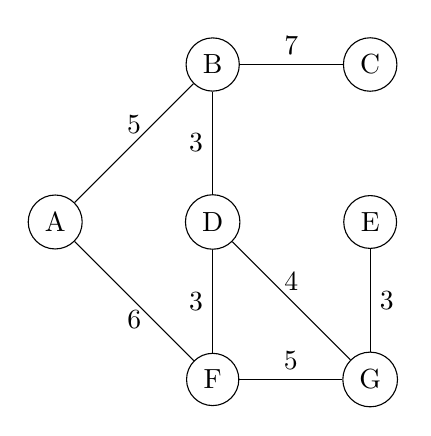
\begin{tikzpicture}
        % Nodi
        \node[circle, draw] (A) at (0,0) {A};
        \node[circle, draw] (B) at (2,2) {B};
        \node[circle, draw] (D) at (2,0) {D};
        \node[circle, draw] (F) at (2,-2) {F};
        \node[circle, draw] (C) at (4,2) {C};
        \node[circle, draw] (G) at (4,-2) {G};
        \node[circle, draw] (E) at (4,0) {E};
    
        % Archi
        \draw[-] (A) -- (B) node[midway, above] {5}; % Arco da A a B
        \draw[-] (A) -- (F) node[midway, below] {6}; % Arco da B a D
        \draw[-] (B) -- (D) node[midway, left] {3}; % Arco da D a C
        \draw[-] (D) -- (F) node[midway, left] {3}; % Arco da C a A
        \draw[-] (B) -- (C) node[midway, above] {7}; % Arco da C a A
        \draw[-] (D) -- (G) node[midway, above] {4}; % Arco da C a A
        \draw[-] (F) -- (G) node[midway, above] {5}; % Arco da C a A
        \draw[-] (G) -- (E) node[midway, right] {3}; % Arco da C a A
    
    \end{tikzpicture}
\end{center}

I vari algoritmi che presenteremo differiscono per come rispondono alla domanda: "\textit{Dato che ho ispezionato il nodo, proseguo o vado indietro?}"


\subsection{Ricerca Non Informata}
\subsubsection{Depth-First-Search}
Un algoritmo classico di ricerca su grafo è la ricerca in profondità. In questa versione, la DFS è dotata di \textit{Backtracking}. Possiamo 
dire in generale che l'approccio di questo algoritmo è aggressiva, poichè ricerca subito in profondità la soluzione (potrebbe metterci molto o potrebbe metterci poco), ossia non c'è garanzia.
Inoltre possiamo osservare che gli alberi generati dalla DFS sono stretti e lunghi.\\
\smallskip
\textbf{Funzionamento:}
\begin{enumerate}
    \item Si parte dal nodo iniziale A (che sarà poi radice dell'albero finale)
    \item Se il nodo da esplorare ha dei figli, si aggiungono all'albero i vari figli; in caso ve ne sia più di uno,
    un \textit{Tie-Breaker} spesso usato è basato sull'ordine lessicografico (quindi, per esempio, se esploriamo A, il primo figlio da esplorare sarà B)
    \item Si torna indietro se: il nodo è foglia, oppure se il nodo è già stato visitato
\end{enumerate}

\textbf{Analisi}:
\begin{itemize}
    \item \textbf{Correttezza}: La dfs restituisce sempre un albero (grazie all'uso del Backtracking e all'eliminazione dei loop)
    \item \textbf{Completezza}: La dfs restituisce sempre un albero in cui un ramo contiene lo stato obiettivo (se esiste il percorso)
    \item \textbf{Complessità Temporale}: Dato b il \textit{Branching Factor} e d la \textit{profondità massima}, la complessità di tale algoritmo è esponenziale, ossia $O(b^d)$
    \item \textbf{Complessità Spaziale}: La memoria usata è quella necessaria per generare l'albero; in questo caso la complessità è $O(d)$ ossia la profondità massima del percorso dallo start al goal.

\end{itemize}

\subsubsection{Breath-First-Search}
Un altro algoritmo classico di ricerca su grafo è la ricerca in ampiezza. Anche la BFS è dotata di \textit{Backtracking}. Possiamo 
dire in generale che l'approccio di questo algoritmo è conservativa, poichè ricerca sempre allo stesso livello, garantendo di visitare tutti i nodi.
Possiamo inoltre dire che gli alberi generati dalla BFS sono larghi e corti.\\
\smallskip
\textbf{Funzionamento:}
\begin{enumerate}
    \item Si parte dal nodo iniziale A (che sarà poi radice dell'albero finale)
    \item Se il nodo padre ha dei figli da esplorare, vengono tutti aggiunti all'albero; Si prosegue poi ai figli del primo nodo figlio e così via.
    Il \textit{Tie-Breaker} che possiamo usare è ancora quello basato sull'ordine lessicografico.
    \item Si torna indietro se: il nodo è foglia, oppure se il nodo è già stato visitato
\end{enumerate}

\textbf{Analisi}:
\begin{itemize}
    \item \textbf{Correttezza}: Per lo stesso motivo della DFS
    \item \textbf{Completezza}: Per lo stesso motivo della DFS
    \item \textbf{Complessità Temporale}: Dato b il \textit{Branching Factor} e q la \textit{profondità minima}, la complessità di tale algoritmo è esponenziale, ossia $O(b^q)$ (quindi sempre minore, nel caso peggiore, della DFS)
    \item \textbf{Complessità Spaziale}: In questo caso, dato che non viene allocata altra memoria se non il grafo stesso, la complessità spaziale sarà $O(n)$ con n il numero di nodi. 
\end{itemize}
\subsubsection{DFS/BFS Ottimizzati}
Gli ultimi 2 algoritmi possono essere ottimizzati introducendo nuove strutture dati, usate per evitare di rivisitare 
i nodi e quindi per generare alberi più piccoli:

\paragraph{EQL (Enqueued List).}
La EQL, anche detta \textit{lista di accodamento}, è una lista che tiene traccia di tutti i nodi già visitati; è detta
di accodamento perchè ad ogni nuova visita, il nodo visitato viene aggiunto alla fine; quando si deve vistare un nodo
si verifica che questo non sia già nella lista; se lo è, tutto il sottoalbero relativo non verrà esplorato. Questa 
operazione è detta \textbf{Potatura} o \textbf{Pruning}

\paragraph{Frontiera.}
Definiamo frontiera l'insieme dei nodi foglia non ancora espansi dell'albero; è detta così dal momento che, per la
\textbf{Separation Property}, separa la parte dell'albero esplorata da quella ancora non esplorata.\\
Implementazioni della Frontiera:
\begin{itemize}
    \item \textbf{Caso BFS}: la frontiera viene implementata come \textbf{Queue} (una coda FIFO)
    \item \textbf{Caso DFS}: la frontiera viene implementata come \textbf{Stack} (una coda LIFO)
\end{itemize}

\textbf{Analisi}:
\begin{itemize}
    \item \textbf{Correttezza}: L'uso delle EQL pota solo i sottoalberi già esplorati, per cui la correttezza non viene compromessa
    \item \textbf{Completezza}: L'algoritmo è ancora completo per il motivo precedente
    \item \textbf{Complessità Temporale/Spaziale}: anche se abbiamo introdotto queste strutture dati per ottimizzare le operazioni,
          in realtà la complessità nel caso peggiore non cambia. Grazie a queste ottimizzazioni, tuttavia, è possibile usare in un tempo ragionevole
          i 2 algoritmi
\end{itemize}

\newpage
\subsection{UCS (Uniform Cost Search)}\lezione{Lezione 5}{14/10/2024}
Nella presentazione di BFS e DFS, abbiamo sempre ipotizzato di dover risolvere problemi di Fattibilità (paragrafo \ref{def:fattibilità}),
per cui i 2 algoritmi hanno dovuto solo esplorare il grafo fino a generare un nodo obiettivo del problema.
Per risolvere il problema di Ottimizzazione, invece, dovremo utilizzare l'approccio conservativo della BFS per progettare 
un algoritmo che trovi sempre il percorso ottimo.\\

\paragraph{Cost To Go Function. }
Per descrivere l'implementazione della UCS è necesasario innanzitutto definire la \textit{Cost-to-Go Function} $g(V)$.
Dato un vertice $V$, $g(V)$ è il costo complessivo per arrivare dallo stato $A$ allo stato $V$ tramite un percorso $p$.

\subsubsection{Algoritmo (Ad alto livello)}
Inizialmente si aggiunge alla Frontiera il nodo di Partenza $A$ e dopodichè
\begin{itemize}
    \item Si calcolano per ogni nodo della frontiera il $g(V)$
    \item Si seleziona il nodo da espandere con $g(V)$ più piccolo
    \item Ci si ferma solo quando \textbf{espandiamo} un nodo Goal
\end{itemize}

\newpage

\subsubsection{Ottimalità di UCS}
Si può dimostrare che UCS non solo è \textbf{corretto} e \textbf{completo} e che seleziona il percorso \textbf{ottimo}, ma che
\textit{"Ogni volta che UCS seleziona per la prima volta un nodo per l'espansione, il percorso che porta ha quel nodo ha costo minimo"}

\paragraph{Ipotesi. }
\begin{enumerate}
    \item UCS seleziona sempre per la prima volta dalla frontiera un nodo $V$ da espandere ottenuto tramite percorso $p$ con costo minore
    \item Il percorso $p$ non è ottimo
\end{enumerate}

\paragraph{Dimostrazione. }
Se $p$ non è ottimo, allora deve esistere sulla frontiera un nodo $X$ tale che la somma dei percorsi $p_1^* = A \longrightarrow X$ e $p_2^* = X \longrightarrow V$ sia $p^* = p_1^* + p_2^*$ e $g(p^*) < g(p)$.
Dal momento che $g(p^*) = g(p_1^*) + \Delta p_2^*$ allora $ g(p_1^*) + \Delta p_2^* < g(p)$; $\Delta p_2^*$ è per definizione una quantità non negativa,
dunque $g(p_1^*) < g(p)$, ossia UCS ha selezionato prima un percorso $p$ che è peggiore di $p_1^*$, e ciò porta ad un \textbf{assurdo} perchè noi
abbiamo definito l'algoritmo in maniera diversa, viene violata la prima ipotesi. Allora $p = p*$.


\begin{center}
    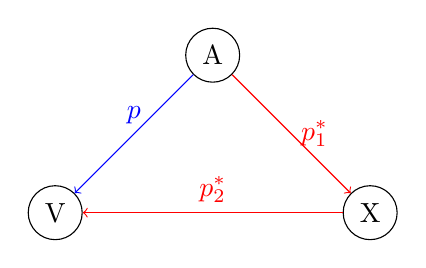
\begin{tikzpicture}
        % Nodi
        \node[circle, draw] (A) at (0,0) {A};
        \node[circle, draw] (V) at (-2,-2) {V};
        \node[circle, draw] (X) at (2, -2) {X};

    
        % Archi
        \draw[->, blue] (A) -- (V) node[midway, above] {$p$}; % Arco da A a B
        \draw[->, red] (A) -- (X) node[midway, right] {$p_1^*$}; % Arco da B a D
        \draw[->, red] (X) -- (V) node[midway, above] {$p_2^*$}; % Arco da D a C

    
    \end{tikzpicture}
\end{center}



\subsubsection{UCS con EXL}
Una prima forma di ottimizzazione della UCS la otteniamo introducendo una struttura dati detta \textit{Expansion List} o \textit{Lista delle Espansioni}
Questa lista è molto simile alla EQL, solo che in questo caso si aggiunge un nodo solo quando deve essere espanso, e non quando viene generato.



\subsection{Ricerca Informata}
Si parla di ricerca \textbf{non informata} quando dobbiamo affrontare un problema di Search avendo a disposizione \textbf{solo} 
il grafo e il criterio di scelta del prossimo nodo da esplorare.\\
Si parla, invece, di ricerca \textbf{informata} quando oltre alle informazioni precedenti abbiamo anche una stima $f(V)$ della bontà
del nodo $V$, ossia quanto è distante tale nodo dall'obiettivo. Tramite queste stime è possibile realizzare algoritmi con approccio
\textbf{Best-First} in cui il criterio di scelta di un nodo da esplorare avviene in base alla minimizzazione di $f(V)$.

\subsubsection{A*}
L'algoritmo A* è un algoritmo nato negli anni '60 per permettere al primo prototipo di Robot autonomo (Shakey) di arrivare da un punto
$A$ ad un punto $B$ col percorso più breve possibile. A* è praticamente identico a UCS, tranne per il fatto che il cost-to-go da ottimizzare è 
$f(s) = g(s) + h(s) $ dove $h(s)$ è detta \textbf{euristica di distanza} dall'ottimo. 
L'euristica dev'essere una funzione:
\begin{itemize}
    \item Computabile in tempo costante
    \item Ammissibile (ossia deve sottostimare il vero valore, o meglio la stima dev'essere ottimista)
\end{itemize} 
Trovare un'euristica sensata al problema, tuttavia, potrebbe non essere semplice.



\subsubsection{A* con EXL}
\lezione{Lezione 6}{17/10/2024}
Dal momento che A* può essere visto come una generalizzazione di UCS (UCS è il caso in cui l'euristica è sempre nulla), possiamo
equipaggiare anche A* con una lista delle espansioni per ottimizzare il tempo di ricerca. Purtroppo, in questo caso, non è sempre detto
che con la EXL e l'euristica si conservi sempre l'ottimalità (perchè è possibile che si selezionino prima percorsi da espandere più lunghi di altri) ed è
per questo che l'euristica $h$ debba essere anche \textbf{consistente}.

\paragraph{Euristica Consistente}
La consistenza (o monotonicità) di un'euristica è una proprietà più forte dell'ammissibilità (quindi la implica) e afferma che:\\
Dati 2 nodi $V,U$ e un'azione $a$, allora
\begin{equation}
    h(V) \leq c(V,a,U) + h(U) \mbox{  } \forall V,U
\end{equation}
La proprietà può essere interpretata come una disuguaglianza triangolare in questa forma (G è il nodo goal):
\begin{center}
    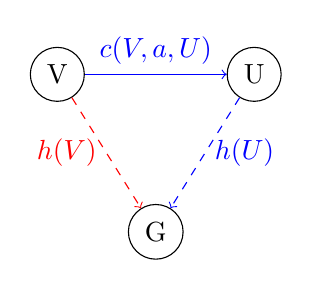
\begin{tikzpicture}
        % Nodi
        \node[circle, draw] (V) at (0,0) {V};
        \node[circle, draw] (U) at (2.5,0) {U};
        \node[circle, draw] (G) at (1.25,-2) {G};

    
        % Archi
        \draw[->, blue] (V) -- (U) node[midway, above] {$c(V,a,U)$}; % Arco da A a B
        \draw[->, dashed, red] (V) -- (G) node[midway, left] {$h(V)$}; % Arco da B a D
        \draw[->, dashed, blue] (U) -- (G) node[midway, right] {$h(U)$}; % Arco da D a C

    
    \end{tikzpicture}
\end{center}
Ossia, la stima di un nodo non può essere peggiore del costo per arrivare al nodo successivo + la stima del nodo successivo.

\subsubsection{Monotonicità di $f$}
Assumendo che $h$ sia consistente, allora possiamo dimostrare che $f$ sia monotona non decrescente.
\paragraph{Dimostrazione. }
Consideriamo i nodi $V,U$ e un arco che li collega $a$ (simili al disegno precedente) generati dopo $p$ passi dall'algoritmo A*.
Sappiamo che $f(U) = g(U) + h(U)$ e che $g(U) = g(V) + c(V,a,U)$; sostituendo otteniamo che $f(U) = h(U) + g(V) + c(V,a,U)$. Allora dalla definizione di consistenza sappiamo che
\begin{align*}
    c(V,a,U) + h(U) &\geq h(V)\\
    \underbrace{h(U) + c(V,a,U) + \textcolor{red}{g(V)}}_{f(U)} &\geq \underbrace{h(V) + \textcolor{red}{g(V)}}_{f(V)} \\
\end{align*}
Dunque
\begin{equation*}
    f(U) \geq f(V)
\end{equation*}

\subsubsection{Ottimalità di A*}
\paragraph{Ipotesi}
\begin{enumerate}
    \item A* seleziona come primo nodo da espandere $V$, ottenuto tramite un percorso $p$
    \item $p$ non è ottimo ($p \neq p^*$)
\end{enumerate}

\paragraph{Dimostrazione}
Se $p$ non è ottimo per ipotesi $2$, allora deve esistere necessariamente sulla frontiera un nodo $X$ che si trova sul cammino ottimo
$p^*$ verso $V$. Lungo ogni percorso, abbiamo dimostrato prima, che f è monotona non decrescente dunque $f(V) \geq f(X)$; allora $V$ non può
essere stato scelto prima di $X$: ASSURDO, $p = p^{*}$

\subsection{Progettare un'Euristica}
\begin{center}
    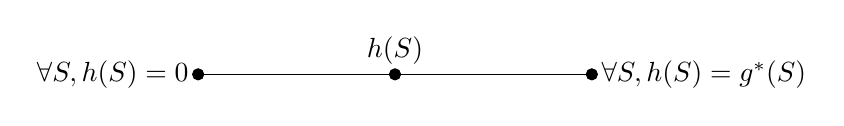
\begin{tikzpicture}
        % Disegna il segmento AB
        \draw[-] (0,0) -- (5,0);
        
        % Punti A, B e C
        \filldraw[black] (0,0) circle (2pt) node[left] {$\forall S, h(S) = 0$}; % Punto A
        \filldraw[black] (5,0) circle (2pt) node[right] {$\forall S, h(S) = g^*(S)$}; % Punto B
        \filldraw[black] (2.5,0) circle (2pt) node[above] {$h(S)$}; % Punto C al centro
    \end{tikzpicture}
\end{center}

Per progettare un'euristica, come abbiamo detto, è necessario non solo che sia ammissibile ma che la sua computazione sia efficiente (computata in tempo costante).
Chiaramente, più è efficiente l'euristica, meno stretta è, quindi dobbiamo trovare il compromesso giusto per avere una buona euristica.
Tale ha come estremi:
\begin{itemize}
    \item L'Estremo sinistro (caso in cui l'euristica è \textbf{triviale})
    \item L'Estremo destro (caso in cui è il problema ad essere \textbf{triviale} e l'euristica conosce già il percorso completo)
\end{itemize}
Realizzare una buona euristica per A* ci permette di diminuire di molto la dimensione degli alberi e permette di risparmiare tempo e spazio occupati, quindi il nostro obiettivo è di ottenere 
l'euristica migliore, ossia:\\
Dati $h_1, h_2 $ euristiche tali che $\forall S, h_1(S) \leq h_2(S)$ allora $h_2$ domina $h_1$. Inoltre, anche se non per tutti gli S un'euristica domina l'altra,
è possibile creare un'euristica dominante su $h_1, h_2$, ossia:
\begin{equation*}
    h_3 = \max\{h_1, h_2\}
\end{equation*}
Un modo che abbiamo per progettare un'euristica è risolvendo un \textbf{Problema Rilassato}

\subsubsection{Problema Rilassato}
Dato un problema $P$, il suo rilassamento $\hat{P}$ è una sua versione più semplice, ottenuta \textit{rilassando} alcuni suoi vincoli;
per esempio, in una mappa, il problema rilassato della ricerca del percorso l'abbiamo ignorando tutti gli ostacoli, ipotizzando di poter attraversare gli edifici.
Per questo motivo vale che per ogni $S,U$ nodi e $a$ azione:
\begin{equation*}
    \hat{c}(S,a,U) \leq c(S,a,U)
\end{equation*}
Risolvere un problema rilassato può essere una buona euristica.

\subsubsection{Limiti di A*}
Il problema di A* è, essenzialmente, che è troppo rigido: nel caso in cui sulla frontiera vi siano MOLTI nodi tutti con un valore di $f$
molto simile, allora A* perderà molto tempo a espanderli tutti quanti. Può essere anche che un nodo arrivi all'ottimo in un certo numero di passi,
mentre un altro nodo ci arrivi con un numero di passi decisamente inferiore. La formulazione di A* più flessibile è il \textbf{Focal Search}

\subsection{Focal Search}
Per l'implementazione del Focal Search è necessario implementare una nuova euristica $\hat{h_F}(n)$ che stima il costo \textbf{computazionale} (e non in termini di passi)
per raggiungere un goal. Questa euristica poi, rispetto all'euristica $h$, deve \textbf{sovrastimare} (quindi essere pessimista).
Possiamo risolvere diversi problemi NP-HARD con questa tecnica (vedi il TSP, potrebbe chiederlo all'esame)

\end{document}